\documentclass[en,11pt,english,black,simple,device=ppt]{elegantbook}

\def\mainclass{main}

\title{Some}
% \subtitle{数字设计初步}

\author{Pannenets.F}
% \institute{微电子学院}
\date{\today}
% \version{4}
% \bioinfo{分类}{笔记}

\extrainfo{Je reviendrai et je serai des millions. —— <<Spartacus>>}
\setcounter{tocdepth}{3}

\lstset{
  mathescape = false}
% \logo{logo-blue.png}
% \cover{logo.jpg}

% 微分号
\newcommand{\dd}[1]{\mathrm{d}#1}
\newcommand{\pp}[1]{\partial{}#1}

\newcommand{\homep}[1]{\section*{Problem #1}}

% FT LT ZT
\newcommand{\ft}[1]{\mathscr{F}[#1]}
\newcommand{\fta}{\xrightarrow{\mathscr{F}}}
\newcommand{\lt}[1]{\mathscr{L}[#1]}
\newcommand{\lta}{\xrightarrow{\mathscr{L}}}
\newcommand{\zt}[1]{\mathscr{Z}[#1]}
\newcommand{\zta}{\xrightarrow{\mathscr{Z}}}

% 积分求和号

\newcommand{\dsum}{\displaystyle\sum}
\newcommand{\aint}{\int_{-\infty}^{+\infty}}

% 简易图片插入
\newcommand{\qfig}[3][nolabel]{
  \begin{figure}[!htb]
      \centering
      \includegraphics[width=0.6\textwidth]{#2}
      \caption{#3}
      \label{\chapname :#1}
  \end{figure}
}

% 表格
\renewcommand\arraystretch{1.5}


% 日期


\begin{document}

\maketitle
\frontmatter

\mainmatter

\section{chap1}


\includepdf[pages=-]{book/Chapter_01.pdf}

\section{chap2}

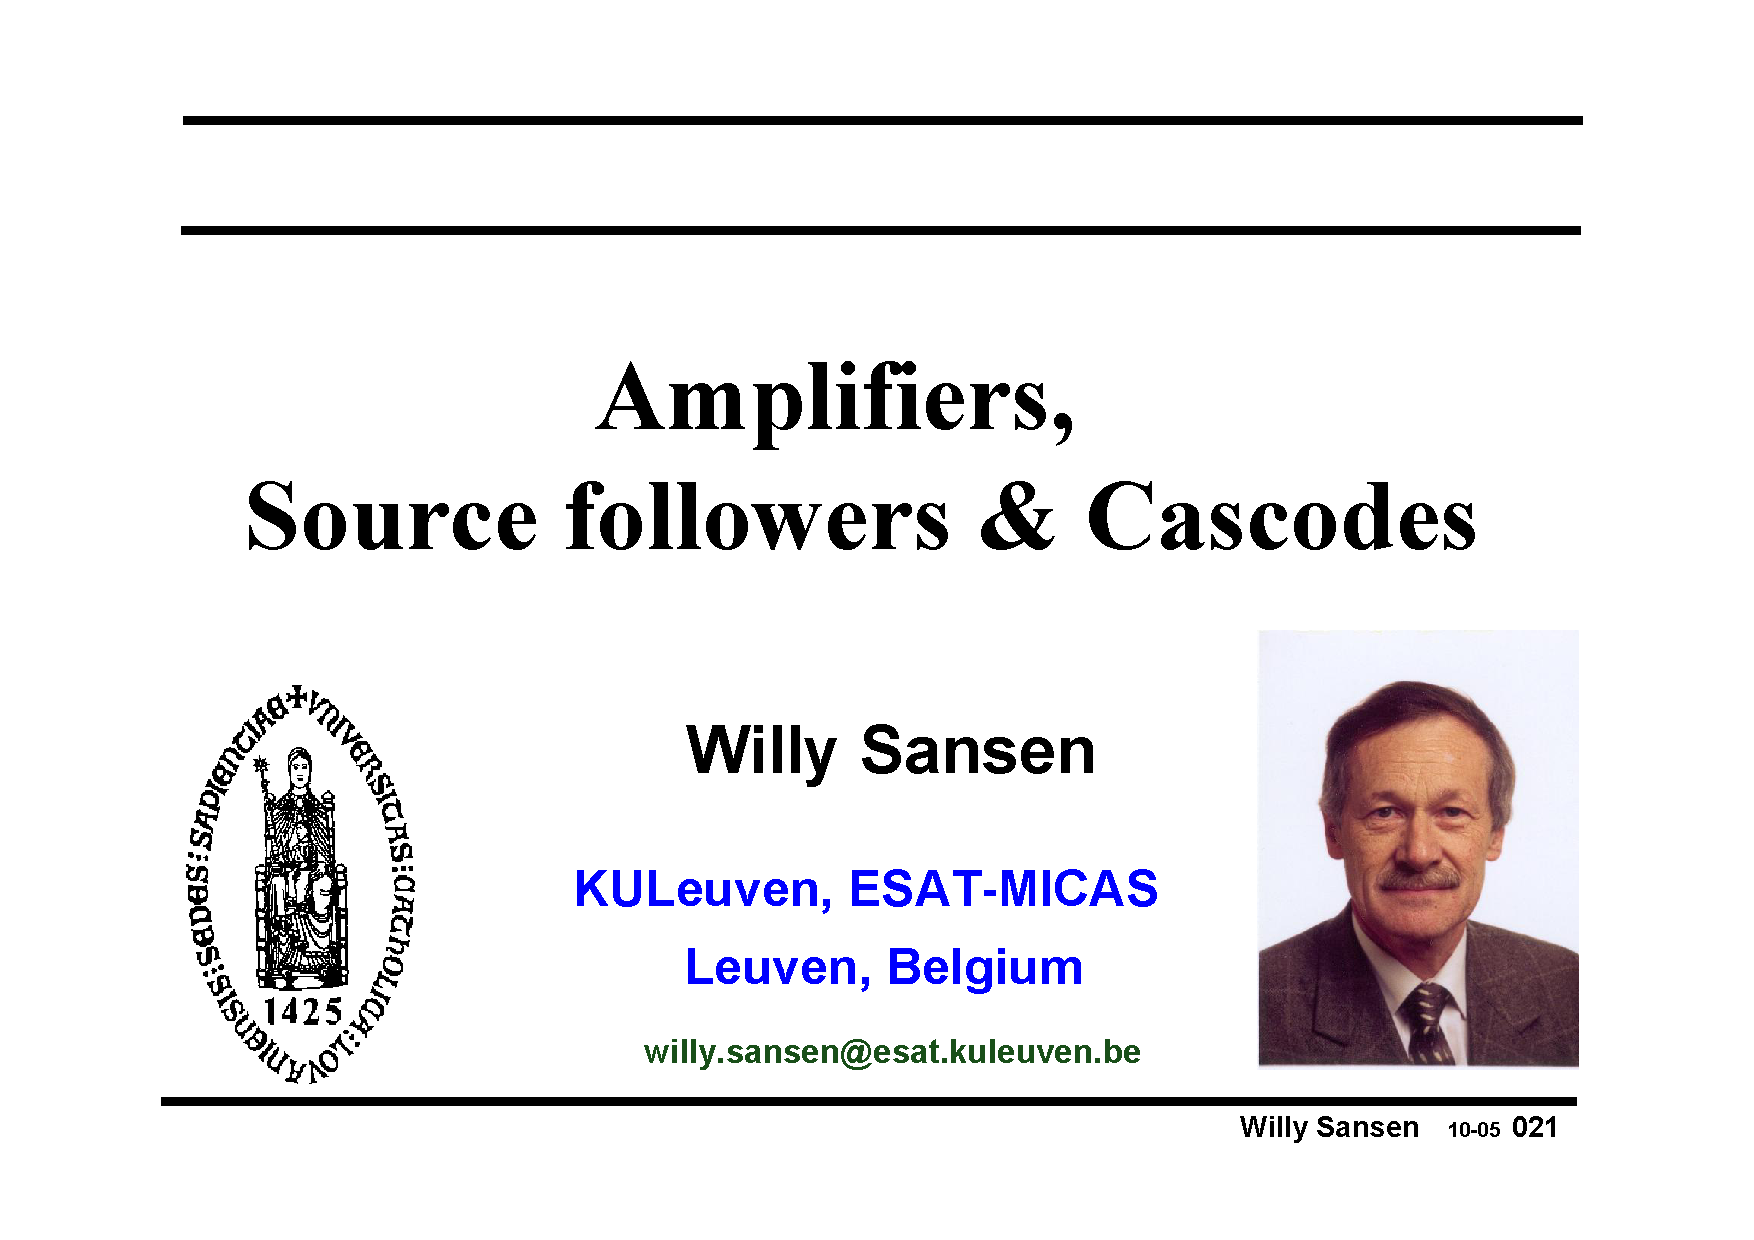
\includepdf[pages=-]{book/Chapter_02.pdf}

\section{chap3}


\includepdf[pages=-]{book/Chapter_03.pdf}

\section{chap4}


\includepdf[pages=-]{book/Chapter_04.pdf}

\section{chap5}


\includepdf[pages=-]{book/Chapter_05.pdf}

\section{chap6}


\includepdf[pages=-]{book/Chapter_06.pdf}

\section{chap7}

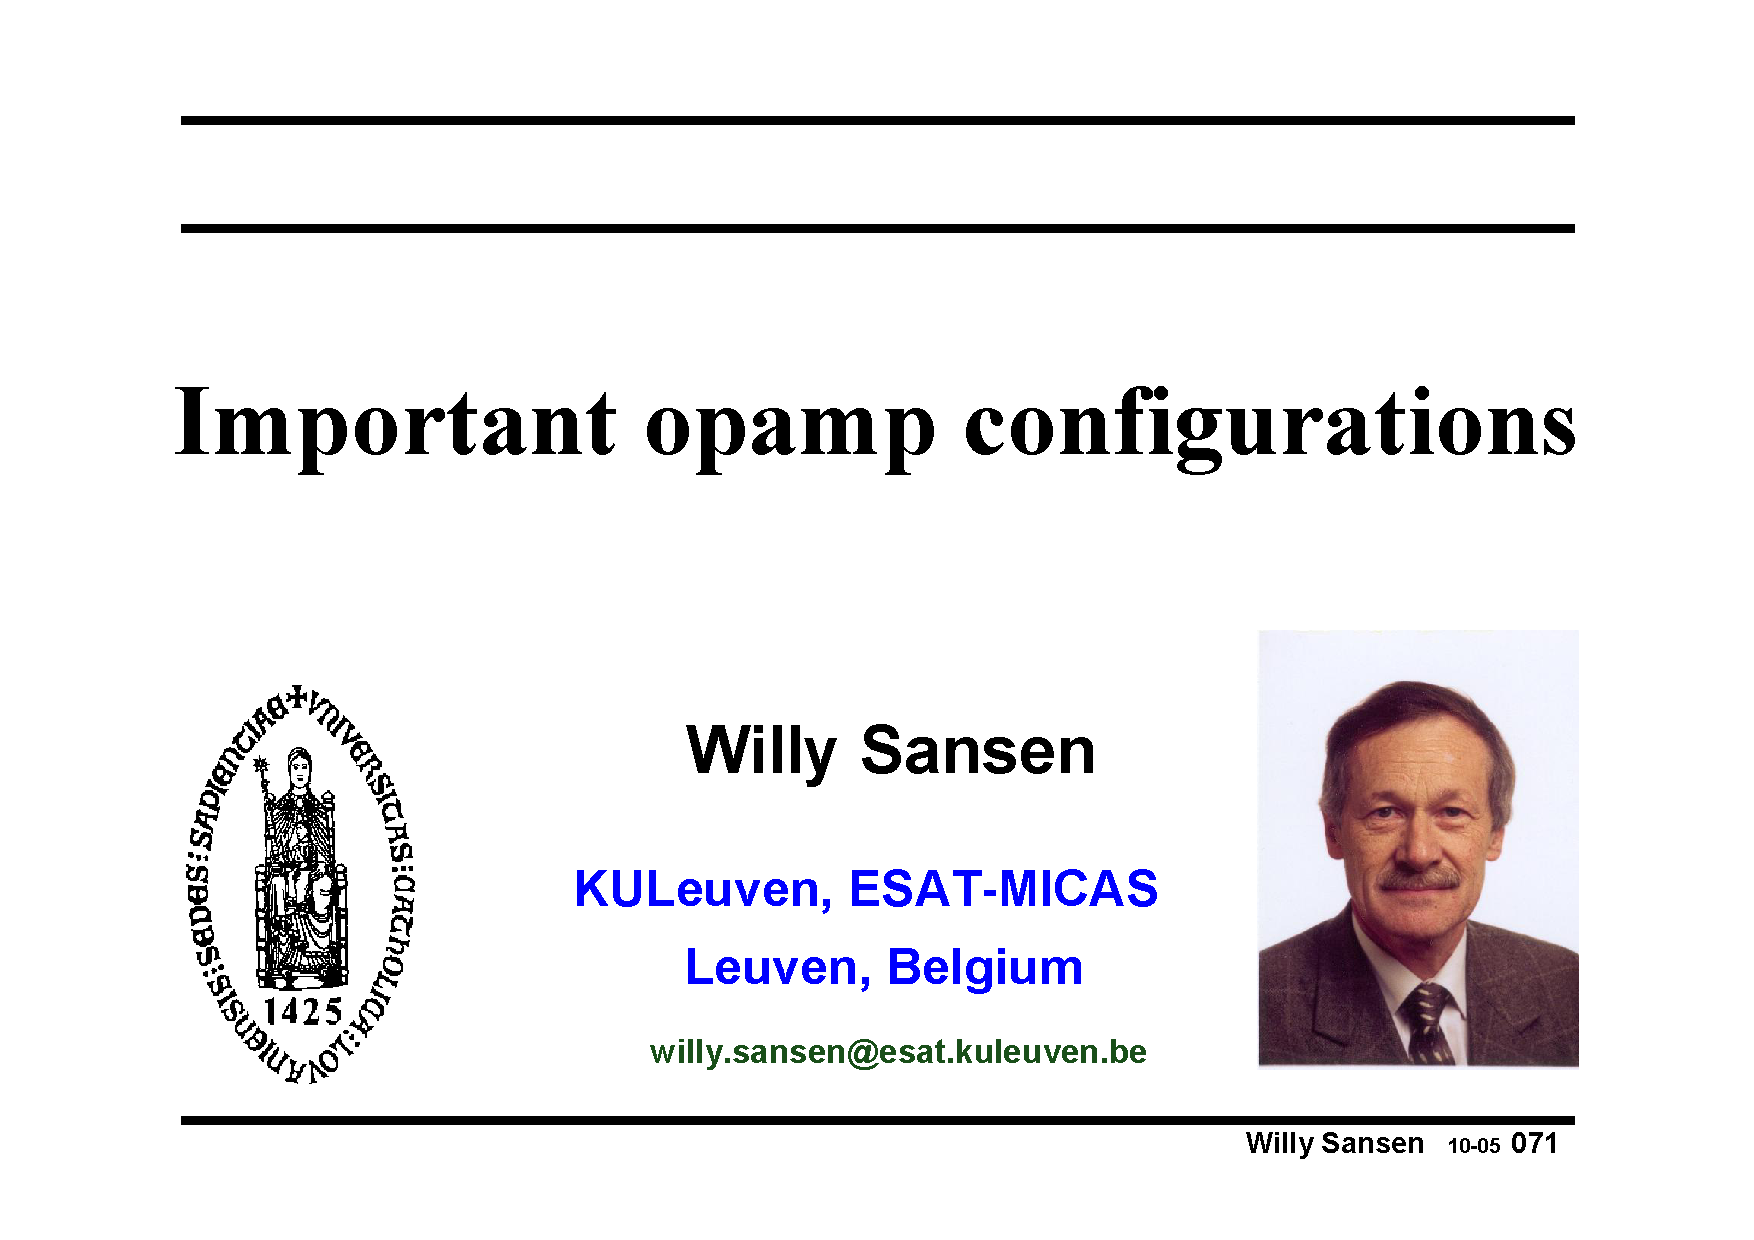
\includepdf[pages=-]{book/Chapter_07.pdf}

\section{chap8}

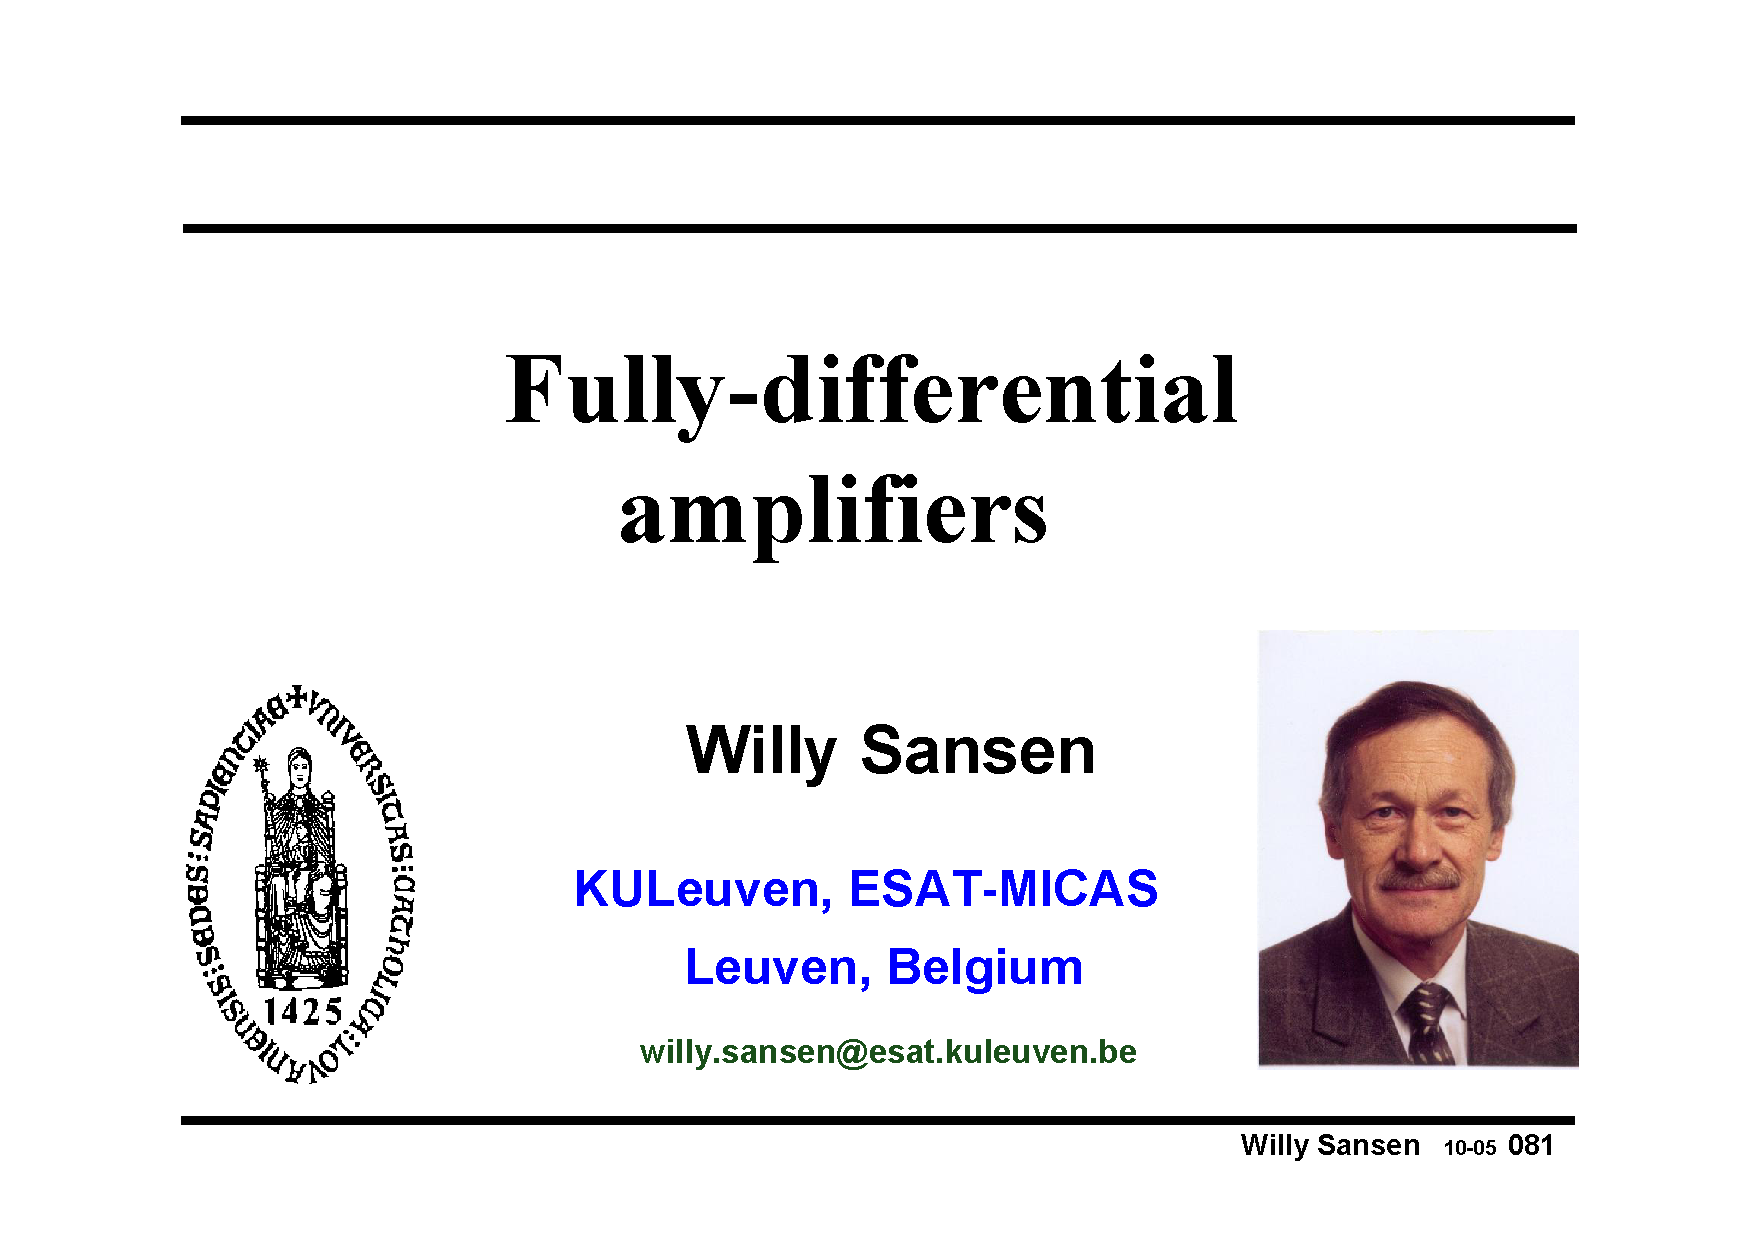
\includepdf[pages=-]{book/Chapter_08.pdf}

\section{chap9}

\includepdf[pages=-]{book/Chapter_09.pdf}

\section{chap10}


\includepdf[pages=-]{book/Chapter_10.pdf}

\section{chap11}

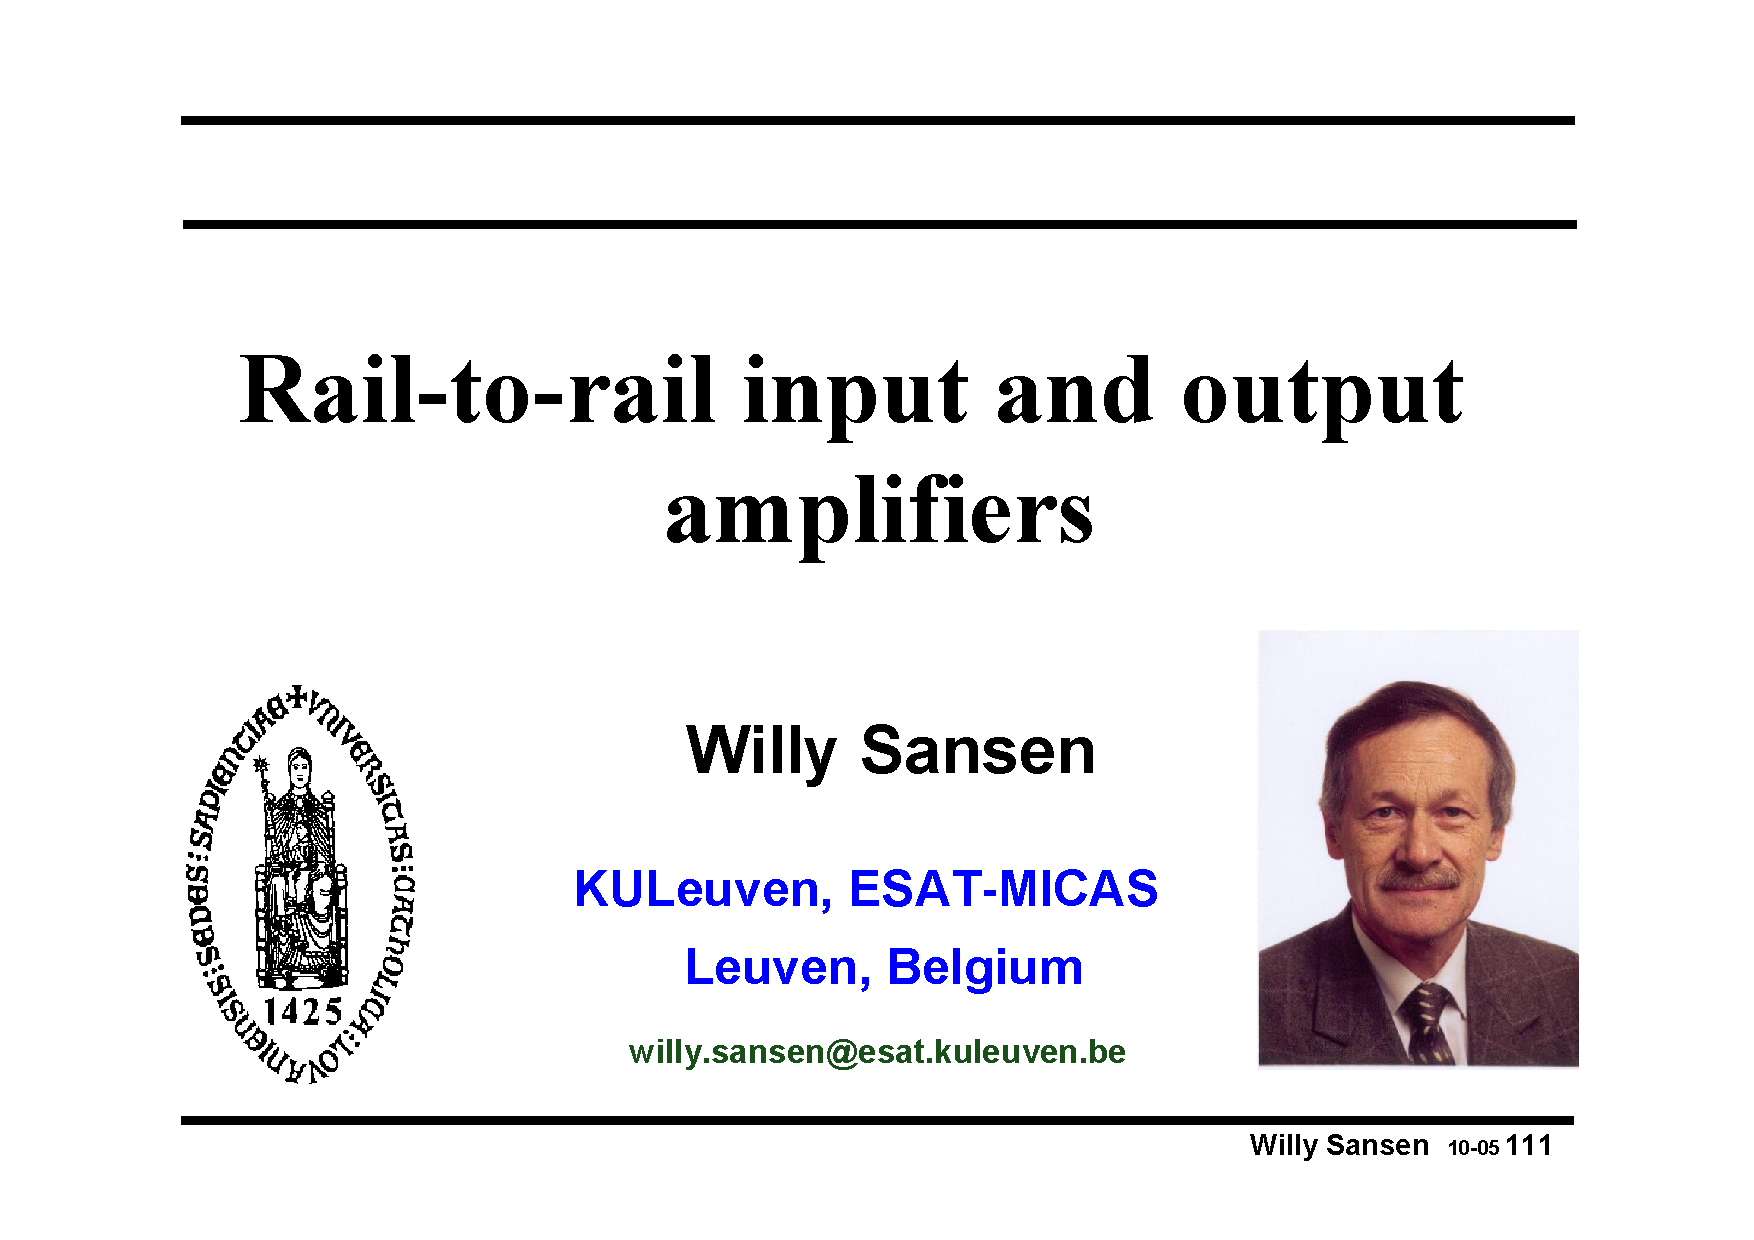
\includepdf[pages=-]{book/Chapter_11.pdf}

\section{chap12}

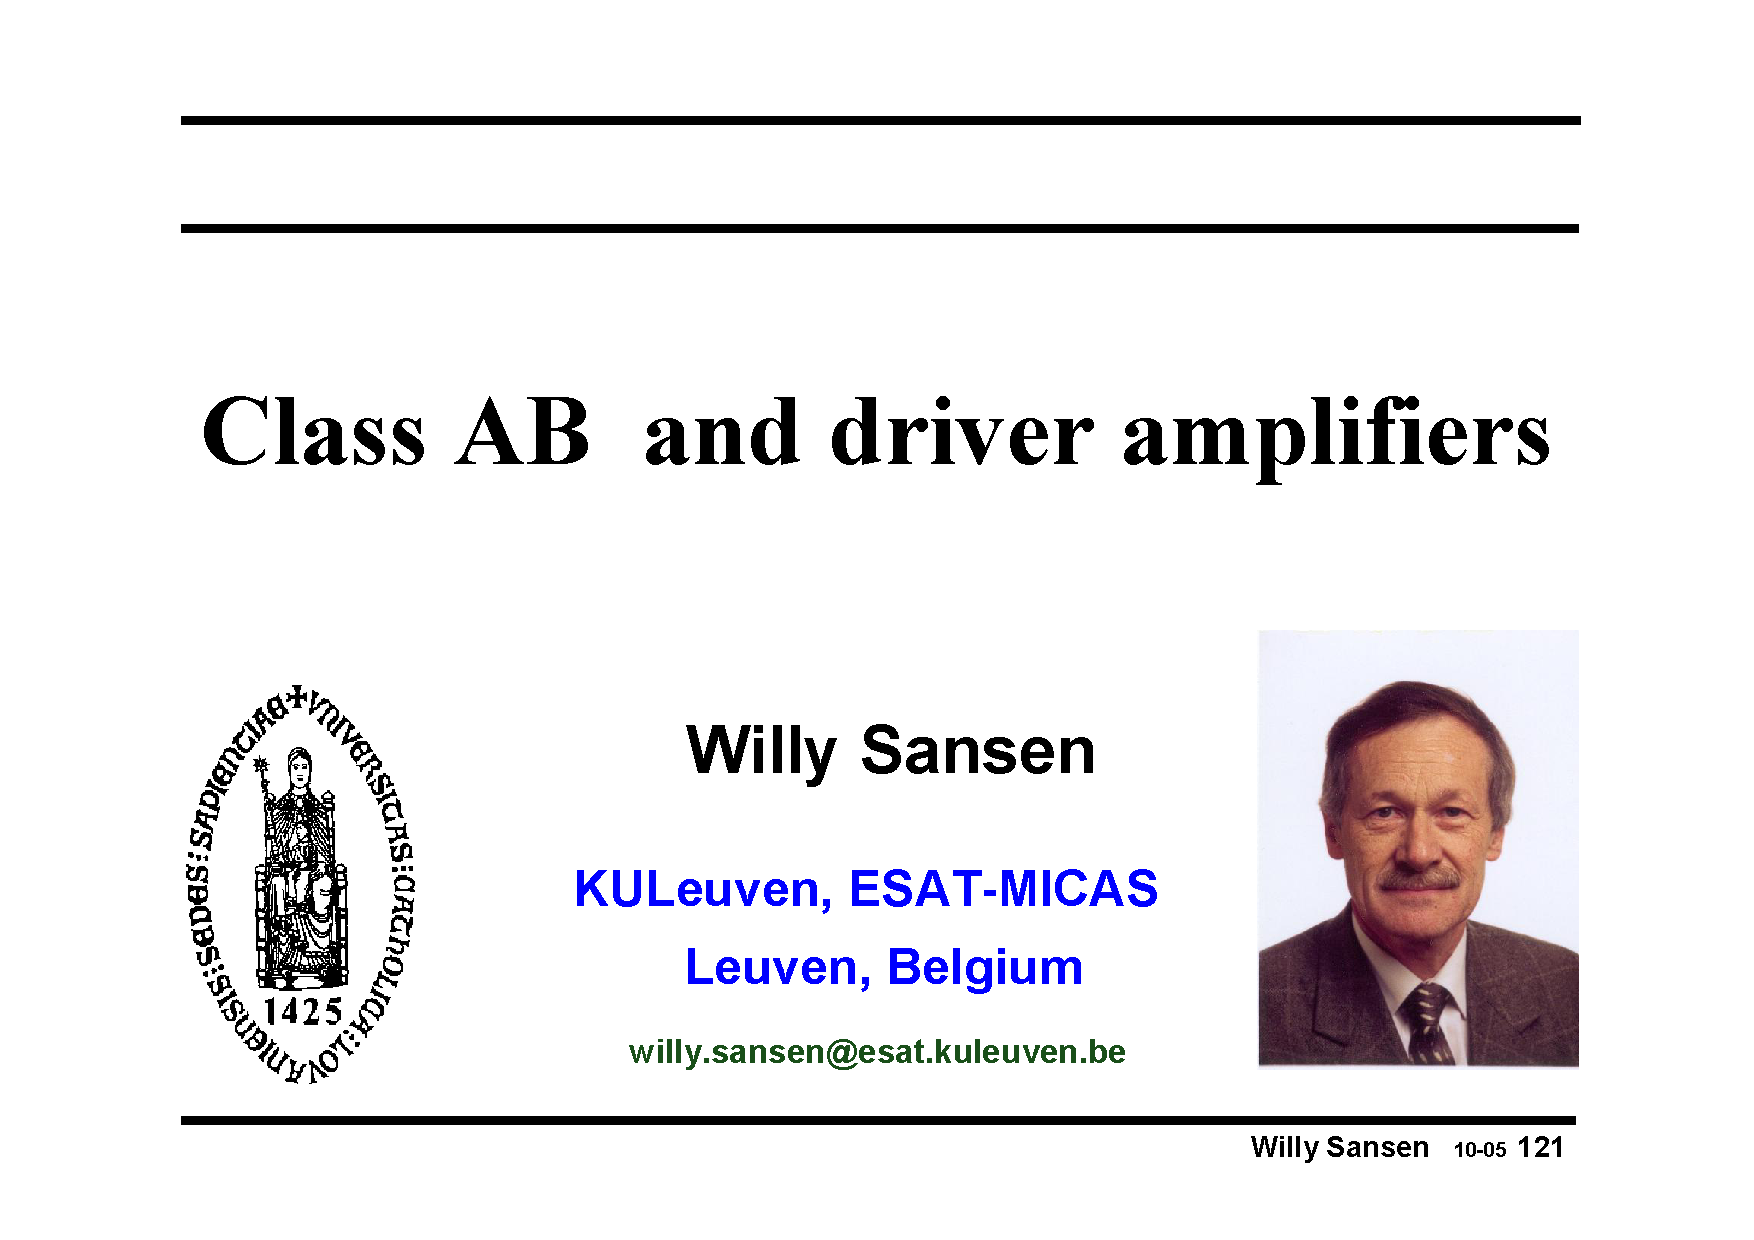
\includepdf[pages=-]{book/Chapter_12.pdf}

\section{chap13}


\includepdf[pages=-]{book/Chapter_13.pdf}

\section{chap14}


\includepdf[pages=-]{book/Chapter_14.pdf}

\section{chap15}


\includepdf[pages=-]{book/Chapter_15.pdf}

\section{chap16}


\includepdf[pages=-]{book/Chapter_16.pdf}

\section{chap17}

\includepdf[pages=1-66]{book/Chapter_177.pdf}

\section{chap18}


\includepdf[pages=-]{book/Chapter_18.pdf}

\section{chap19}

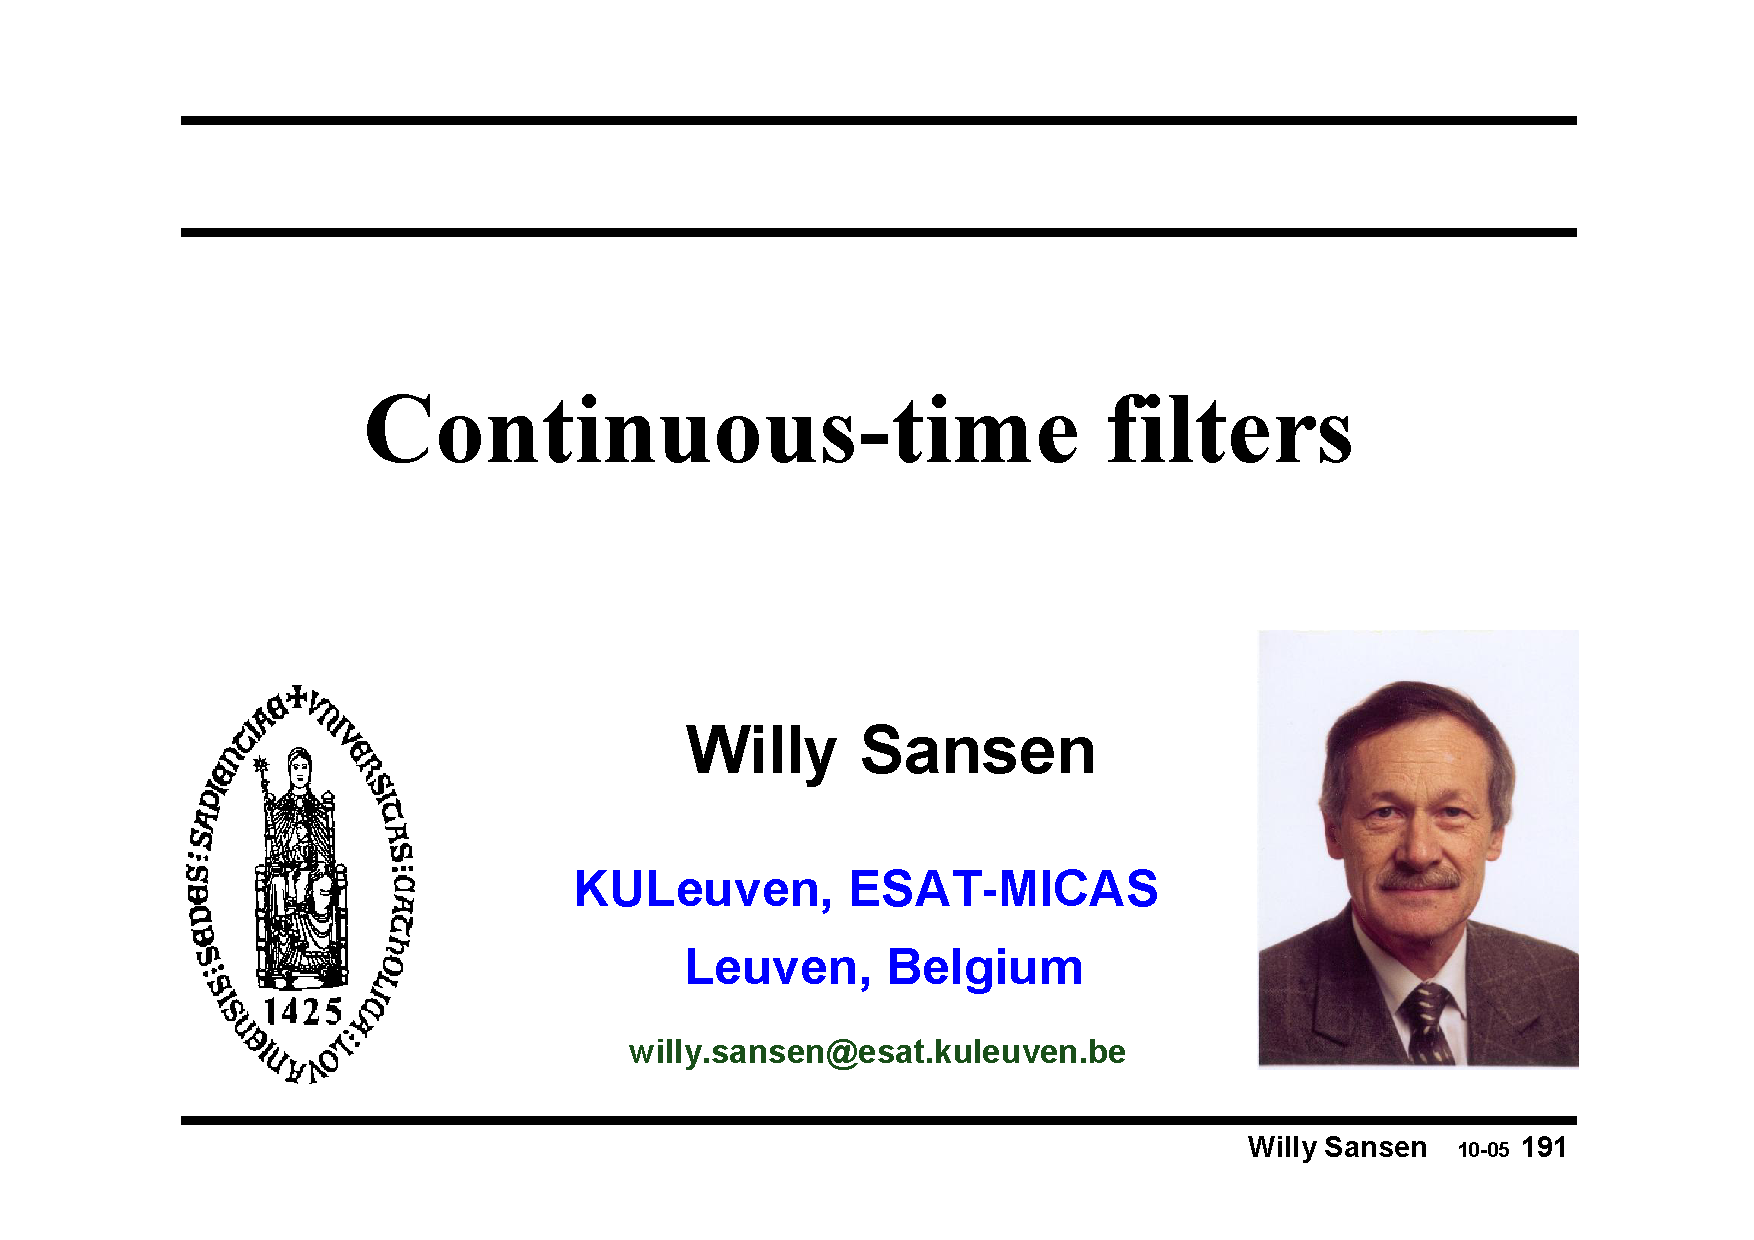
\includepdf[pages=-]{book/Chapter_19.pdf}

\section{chap20}


\includepdf[pages=-]{book/Chapter_20.pdf}

\section{chap21}


\includepdf[pages=-]{book/Chapter_21.pdf}

\section{chap22}

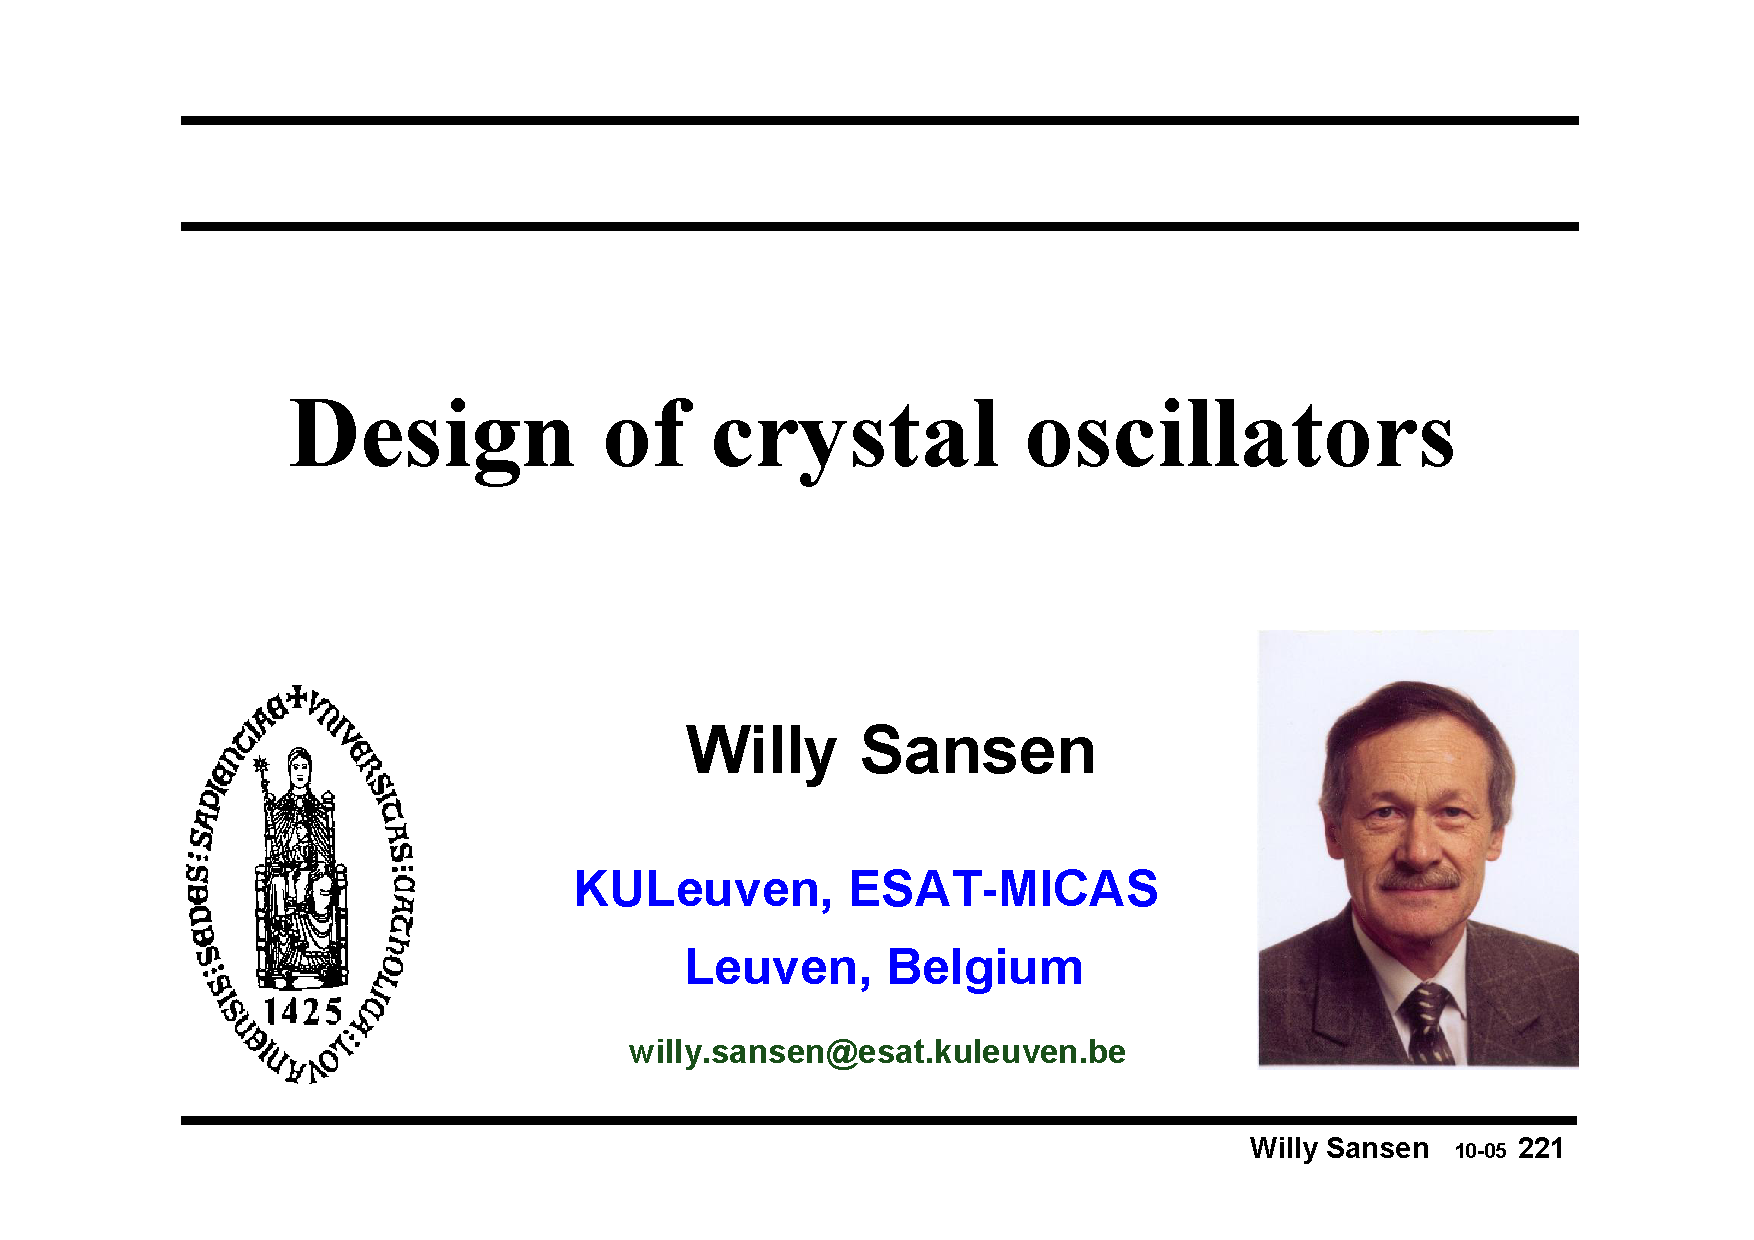
\includepdf[pages=-]{book/Chapter_22.pdf}

\section{chap23}

\includepdf[pages=-]{book/Chapter_23.pdf}

\section{chap24}

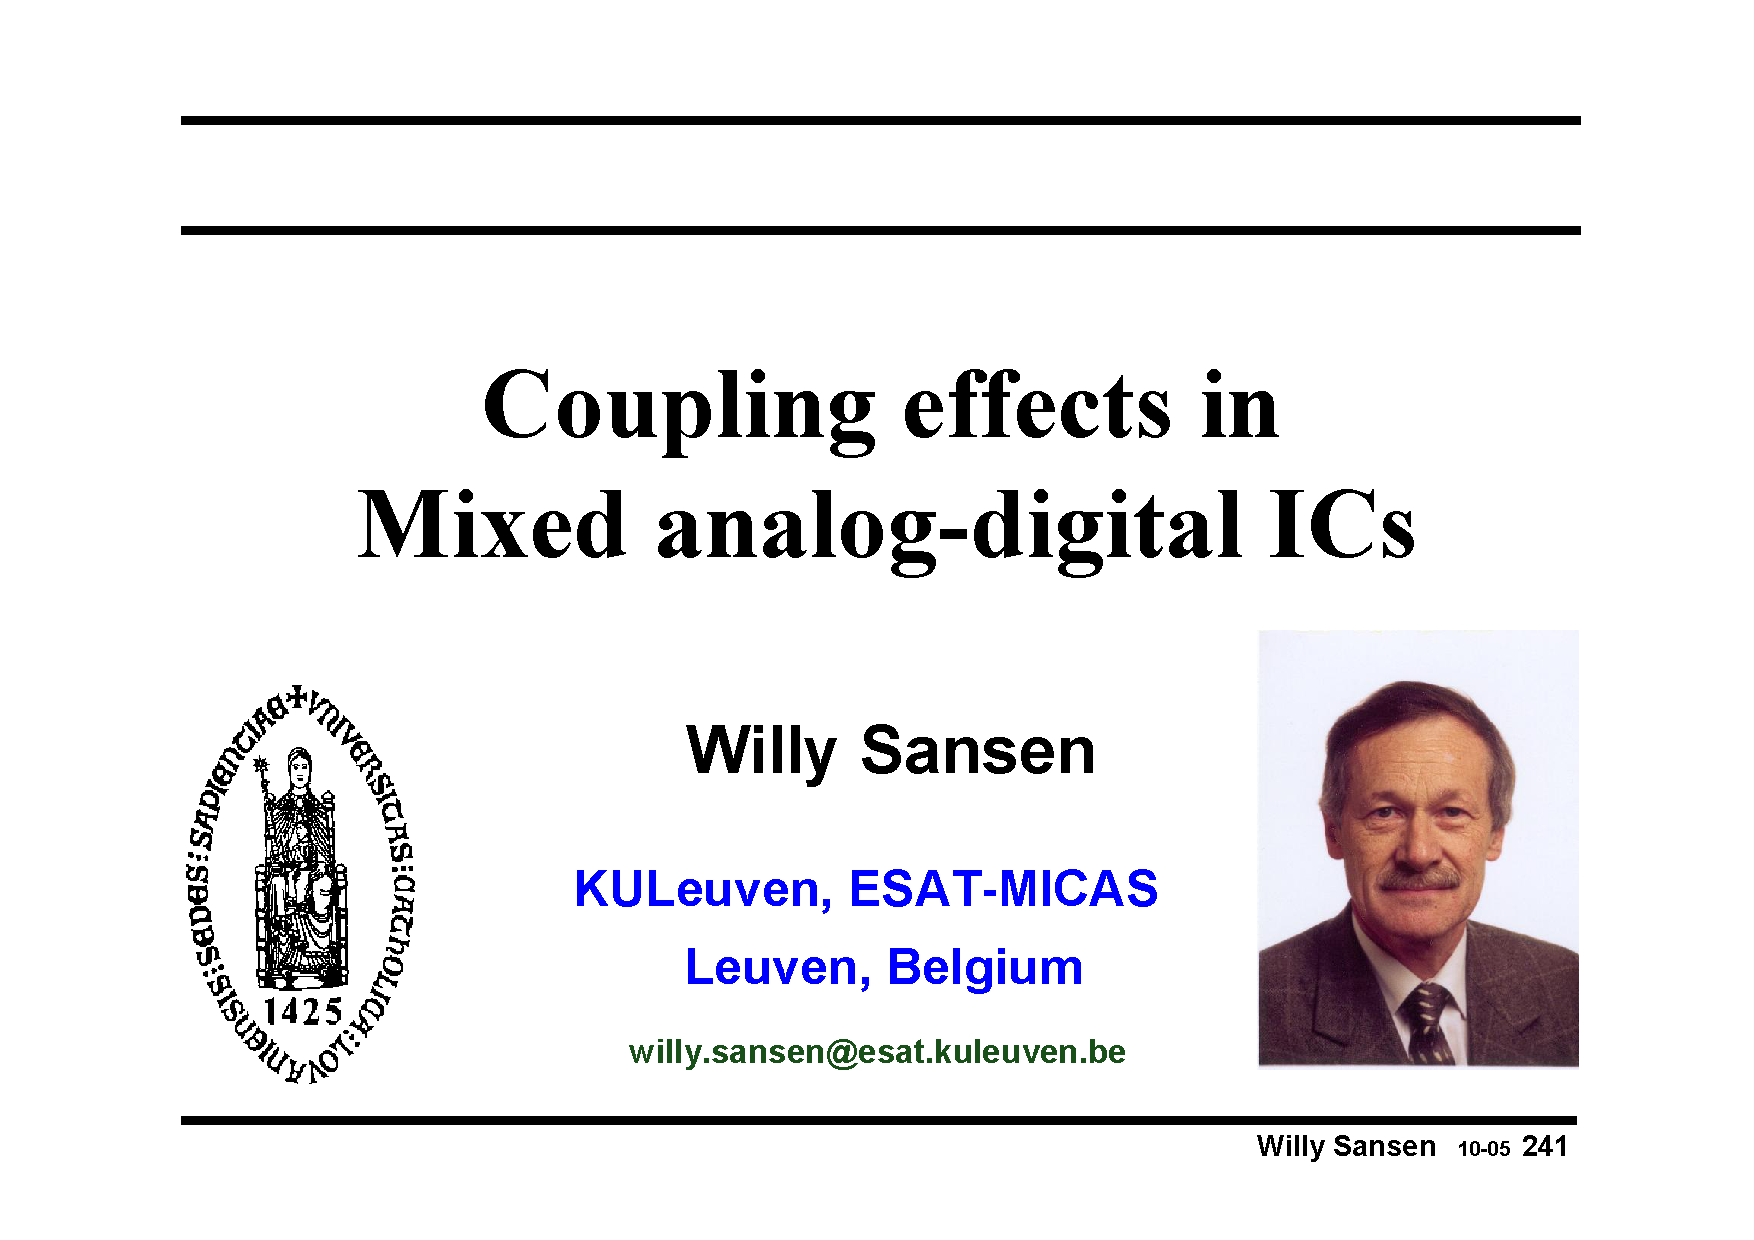
\includepdf[pages=-]{book/Chapter_24.pdf}







\end{document}
